%Este trabalho está licenciado sob a Licença Atribuição-CompartilhaIgual 4.0 Internacional Creative Commons. Para visualizar uma cópia desta licença, visite http://creativecommons.org/licenses/by-sa/4.0/deed.pt_BR ou mande uma carta para Creative Commons, PO Box 1866, Mountain View, CA 94042, USA.

\chapter{Números reais}\label{cap_numreal}
\thispagestyle{fancy}

\section{Conjuntos numéricos}\label{cap_numreal_sec_funconj}

\begin{flushright}
  [Vídeo] | [Áudio] | \href{https://phkonzen.github.io/notas/contato.html}{[Contatar]}
\end{flushright}

\subsection{Definição de conjunto}

\begin{flushright}
  [Vídeo] | [Áudio] | \href{https://phkonzen.github.io/notas/contato.html}{[Contatar]}
\end{flushright}

Um \emph{conjunto} $A$ é uma coleção de elementos ou objetos. Quando $x$ é um \emph{elemento} do conjunto $A$, denotamos
\begin{equation}
  x\in A,
\end{equation}
lê-se \emph{x pertence ao conjunto A}. Já, a notação
\begin{equation}
  x\not\in A
\end{equation}
é usada para denotar que \emph{$x$ não pertence ao $A$}.

Usualmente, um conjunto é descrito usando a notação
\begin{equation}
  A = \{x:~\text{condição para }x\},
\end{equation}
lê-se $A$ é o conjunto dos elementos $x$ tais que $x$ satisfaz a condição.

\begin{ex}
  O conjunto $A$ formado por números positivos pode ser denotado por
  \begin{equation}
    A = \{x: x>0\}.
  \end{equation}
  Ainda, observamos que $2\in A$, $\sqrt{2}\in A$, mas $-1\not\in A$. Você saberia escolher mais elementos que pertençam ou que não pertençam a $A$?

  \ifispython
  No \python, podemos definir este conjunto com
  \begin{lstlisting}
    from sympy import *
    x = Symbol('x')
    A = ConditionSet(x, x>0)
  \end{lstlisting}
  o que nos fornece
  \begin{lstlisting}
    In : 2 in A
    Out: True
    In : sqrt(2) in A
    Out: True
    In : -1 in A
    Out: False
  \end{lstlisting}
  \fi
\end{ex}

\subsubsection{Conjunto finito}

\emph{Conjunto finito} é todo aquele que contém um número finito de elementos. Tais conjuntos podem ser descritos de forma simplificada como segue
\begin{equation}
  A = \{a_1, a_2, \ldots, a_n\},
\end{equation}
neste caso, temos um conjunto com $n$ elementos. Analogamente, um conjunto que contenha infinitos elementos é chamado de \emph{conjunto infinito}.

\begin{obs}
  \begin{equation}
    A = \{-1,3,2\}
  \end{equation}
  é o conjunto que contém apenas os números $-1$, $3$ e $2$.

  \ifispython
  No \python, podemos definir tal conjunto com o seguinte código
  \begin{lstlisting}
    from sympy import *
    A = FiniteSet(-1, 3, 2)
  \end{lstlisting}
  Com este, obtemos
  \begin{lstlisting}
    In : -1 in A
    Out: True
    In : sqrt(2) in A
    Out: False
  \end{lstlisting}
  \fi
\end{obs}

\subsubsection{Conjunto vazio}

O conjunto que não contém elemento algum é chamado de \emph{conjunto vazio} e é denotado por $\emptyset$ ou por $\{\}$.

\begin{ex}
  O conjunto $A$ de todos os números negativos e positivos é vazio, i.e.
  \begin{equation}
    A = \{x: x>0\text{ e }x<0\} = \emptyset
  \end{equation}

  \ifispython
  No \python, podemos definir o conjunto vazio com
  \begin{lstlisting}
    >>> from sympy import *
    >>> A = EmptySet
  \end{lstlisting}
  \fi
\end{ex}

\subsubsection{Igualdade de conjuntos}

Dois \emph{conjuntos} $A$ e $B$ são \emph{iguais}, quando todos os elementos $A$ pertencem a $B$ e vice-versa. Em notação matemática, escrevemos $A=B$ quando
\begin{equation}
  x\in A \Leftrightarrow x\in B,
\end{equation}
lê-se $x\in A$ se, e somente se, $x\in B$.

\begin{ex}
  \begin{enumerate}[a)]
  \item São iguais os conjuntos
    \begin{gather}
      A = \{-1, 3, 2\}\\
      B = \{3, 2, -1\},
    \end{gather}
    i.e. $A = B$.

    \ifispython
    No \python, temos
    \begin{lstlisting}
      from sympy import *
      A = FiniteSet(-1, 3, 2)
      B = FiniteSet(3, 2, -1)
    \end{lstlisting}
    Com este, obtemos
    \begin{lstlisting}
      In : A == B
      Out: True
    \end{lstlisting}
    \fi

  \item São diferentes os conjuntos
    \begin{gather}
      C = \{-3, -2, -1, 0\}\\
      D = \{-3, -1, 0, 2\},
    \end{gather}
    i.e. $C\neq D$.

    \ifispython
    No \python, temos
    \begin{lstlisting}
      from sympy import *
      C = FiniteSet(-3, -2, -1, 0)
      D = FiniteSet(-33, -1, 0, 2)
    \end{lstlisting}
    Com este, obtemos
    \begin{lstlisting}
      In : C != D
      Out: True
    \end{lstlisting}
    \fi
  \end{enumerate}
\end{ex}

\subsubsection{Subconjuntos}

Dizemos que $A$ é subconjunto de $B$, quando todos os elementos de $A$ pertencem a $B$. Neste caso, denotamos
\begin{equation}
  A \subset B
\end{equation}
e lemos ``A está contido em B''. Mais precisamente, $A\subset B$ quando
\begin{equation}
  x\in A \Rightarrow x\in B,
\end{equation}
lemos $x\in A$ implica $x\in B$. O mesmo pode ser denotado por $B\supset A$, i.e. B contém A.

\begin{ex}
  Sejam os seguintes conjuntos
  \begin{gather}
    A = \{-1, 3, 2\}\\
    B = \{2, 3\}.
  \end{gather}
  Temos que $B$ é subconjunto de $A$, i.e. $A\subset B$ ($A$ está contido em $B$).
    
  \ifispython
  No \python, temos
  \begin{lstlisting}
    from sympy import *
    A = FiniteSet(-1, 3, 2)
    B = FiniteSet(2, 3)
  \end{lstlisting}
  Com este, obtemos
  \begin{lstlisting}
    In : B.is_subset(A)
    Out: True
  \end{lstlisting}
  \fi
\end{ex}

\subsection{Operações entre conjuntos}

\begin{flushright}
  [Vídeo] | [Áudio] | \href{https://phkonzen.github.io/notas/contato.html}{[Contatar]}
\end{flushright}

\subsubsection{União de conjuntos}

Sejam $A$ e $B$ dois conjuntos dados. A união do conjunto $A$ com o conjunto $B$ é o conjunto $A\cup B$ que contém todos os elementos de $A$ e todos os elementos de $B$. Mais precisamente, temos
\begin{equation}
  A\cup B = \{x:~x\in A \text{ ou } x\in B\},
\end{equation}
lê-se o conjunto dos elementos $x$ tais que $x\in A$ ou $x\in B$.

\begin{ex}
  Se
  \begin{gather}
    A = \{-1, 3, 2\}\\
    B = \{-2, 0\},
  \end{gather}
  então
  \begin{equation}
    A\cup B = \{-2, -1, 0, 2, 3\}.
  \end{equation}

  \ifispython
  No \python, temos
  \begin{lstlisting}
    from sympy import *
    A = FiniteSet(-1, 3, 2)
    B = FiniteSet(-2, 0)
  \end{lstlisting}
  \begin{lstlisting}
    In : Union(A, B)
    Out: FiniteSet(-2, -1, 0, 2, 3)
  \end{lstlisting}
  \fi
\end{ex}

\subsubsection{Interseção de conjuntos}

Sejam $A$ e $B$ dois conjuntos dados. A interseção do conjunto $A$ com o conjunto $B$ é o conjunto $A\cap B$ que contém os elementos que pertencem simultaneamente a ambos os conjuntos $A$ e $B$. Mais precisamente, temos
\begin{equation}
  A\cap B = \{x:~x\in A \text{ e } x\in B\},
\end{equation}
lê-se o conjunto dos elementos $x$ tais que $x\in A$ e $x\in B$.

\begin{ex}
  Se
  \begin{equation}
    A = \{-1, 3, 2\}\\
    B = \{3, 0\},
  \end{equation}
  então
  \begin{equation}
    A\cap B = \{3\}.
  \end{equation}

  \ifispython
  No \python, temos
  \begin{lstlisting}
    from sympy import *
    A = FiniteSet(-1, 3, 2)
    B = FiniteSet(3, 0)
  \end{lstlisting}
  \begin{lstlisting}
    In : Intersection(A, B)
    Out: FiniteSet(3)
  \end{lstlisting}
  \fi
\end{ex}

\subsubsection{Diferença entre conjuntos}

Sejam $A$ e $B$ dois conjuntos dados. A diferença (ou complemento relativo) do conjunto $A$ com o conjunto $B$ é o conjunto $A\setminus B$ que contém os elementos que pertencem ao $A$ e não pertencem ao conjunto $B$. Mais precisamente, temos
\begin{equation}
  A\setminus B = \{x:~x\in A \text{ e } x\not\in B\},
\end{equation}
lê-se o conjunto dos elementos $x$ tais que $x\in A$ e $x\not\in B$.

\begin{ex}
  Se
  \begin{gather}
    C = \{-3, -2, -1, 0\}\\
    D = \{-3, -1, 0, 2, 4\},
  \end{gather}
  então
  \begin{equation}
    C\setminus D = \{-2\}.
  \end{equation}

  \ifispython
  No \python, temos
  \begin{lstlisting}
    from sympy import *
    C = FiniteSet(-3,-2,-1,0)
    D = FiniteSet(-3,-1,0,2,4)
  \end{lstlisting}
  \begin{lstlisting}
    In : C - D
    Out: FiniteSet(-2)
  \end{lstlisting}
  \fi
\end{ex}

\subsubsection{Produto cartesiano}

Sejam $A$ e $B$ dois conjuntos. O produto cartesiano de $A$ com $B$ é o conjunto $A\times B$, cujos elementos são os \emph{pares ordenados} $(x, y)$ com $x\in A$ e $y\in B$. Mais precisamente, temos
\begin{equation}
  A\times B = \{(x, y):~x\in A \text{ e } y\in B\},
\end{equation}
lê-se o conjunto dos pares ordenados $(x, y)$ tais que $x\in A$ e $x\in B$.

\begin{obs}
  Um par ordenado $(x, y)$ é um conjunto formado por $x$ e $y$, no qual a posição dos elementos importa. Por exemplo, temos
  \begin{equation}
    (3, -1) \neq (-1, 3),
  \end{equation}
  enquanto que
  \begin{equation}
    \{3, -1\} = \{-1, 3\}.
  \end{equation}

  \ifispython
  No \python, escrevemos
  \begin{lstlisting}
    from sympy import *
    A = (3, -1)
    B = (-1, 3)
  \end{lstlisting}
  então
  \begin{lstlisting}
    In : A = (3, -1)
    In : B = (-1, 3)
    In : A == B
    Out: False
  \end{lstlisting}
  \fi
\end{obs}

\begin{ex}
  Se
  \begin{gather}
    A = \{-3, -2, -1\}\\
    B = \{0, 1\},
  \end{gather}
  então
  \begin{gather}
    A\times B = \{(-3,0), (-2, 0), (-1, 0),\nonumber\\
    (-3, 1), (-2, 1), (-1, 1)\}.
  \end{gather}

  \ifispython
  No \python, temos
  \begin{lstlisting}
    from sympy import *
    A = FiniteSet(-3,-2,-1)
    B = FiniteSet(0, 1)
    C = ProductSet(A, B)
  \end{lstlisting}
  então
  \begin{lstlisting}
    In : (-3, 1) in C 
    Out: True
  \end{lstlisting}
  Ainda, podemos imprimir todos os pares ordenados de $C$ com o seguinte código
  \begin{lstlisting}
    for i,p in enumerate(C):
        print(p)
  \end{lstlisting}
  Verifique!    
  \fi
\end{ex}

\subsection*{Exercícios}

\begin{exer}
  Considere o seguinte conjunto
  \begin{equation}
    D = \{...,-3,-2,-1,0,1,2,3,...\}.
  \end{equation}
  Em cada item, diga se é verdadeira ou falsa a afirmação. Justifique cada resposta.
  \begin{enumerate}[a)]
  \item $-1\in D$
  \item $1\not\in D$
  \item $-5\not\in D$
  \item $\sqrt{100}\not\in D$
  \item $D$ é um conjunto finito
  \end{enumerate}
\end{exer}
\begin{resp}
  a) V; b) V; c) F; d) V; e) F
\end{resp}

\begin{exer}
  Dado $A = \{1, 2, \{3, 4\}, 5\}$, determine se as seguintes afirmações são verdadeiras ou falsas. Justifique sua resposta.
  \begin{enumerate}[a)]
  \item $\{2,5\}\subset A$
  \item $\{2,3\}\not\subset A$
  \item $\{3, 4\}\subset A$
  \item $\{3, 4\}\in A$
  \item $\{2, \{3, 4\}\} \subset A$
  \end{enumerate}
\end{exer}
\begin{resp}
  a) V; b) V; c) F; d) V; e) V
\end{resp}

\begin{exer}
  Determine todos os subconjuntos de
  \begin{equation}
    \{1, -1, 2, -3\}
  \end{equation}
\end{exer}
\begin{resp}
  $\emptyset$, $\{1\}$, $\{-1\}$, $\{2\}$, $\{-3\}$, $\{1,-1\}$, $\{1,2\}$, $\{1,-3\}$, $\{-1,2\}$, $\{-1,-3\}$, $\{2,-3\}$, $\{1,-1,2\}$, $\{1,-1,-3\}$, $\{1,2,-3\}$, $\{-1,2,-3\}$, $\{1,-1,2,-3\}$
\end{resp}

\begin{exer}
  Responda cada um dos seguintes itens:
  \begin{enumerate}[a)]
  \item Quantos subconjuntos tem um conjunto de 5 elementos.
  \item Quantos elementos tem um conjunto que contém exatamente 16 subconjuntos.
  \end{enumerate}
\end{exer}
\begin{resp}
  a) $2^5 = 32$; b) $4$ 
\end{resp}

\begin{exer}
  Sejam os seguintes conjuntos
  \begin{gather}
    C = \{-4,2,-1,0,3\}\\
    D = \{5,-3,2,-4\}
  \end{gather}
  Determine os seguintes conjuntos:
  \begin{enumerate}[a)]
  \item $C\cup D$
  \item $C\cap D$
  \item $C - D$
  \item $D - C$
  \item $C\cup \emptyset$
  \item $D\cap \emptyset$
  \end{enumerate}
\end{exer}
\begin{resp}
  a) $\{-4,-3,-1,0,2,3,5\}$; b) $\{-4,2\}$; c) $\{-1,0,3\}$, d) $\{-3,5\}$; e) $C$; f) $\emptyset$
\end{resp}

\begin{exer}
  Seja $A$ um conjunto com 10 elementos e $B$ outro com 25. Sabendo que $A\cap B$ tem 5 elementos, determine o número de elementos do conjunto $A\cup B$. 
\end{exer}
\begin{resp}
  30
\end{resp}

\begin{exer}
  Sejam $A$ e $B$ conjuntos quaisquer. Diga se é verdadeira ou falsa cada uma das seguintes afirmações. Justifique sua resposta.
  \begin{enumerate}[a)]
  \item $A \subset A\cup B$
  \item $A\cap B \supset A$
  \item $A\cup B \supset B$
  \item $A\cap B \subset A$
  \item $A\cup B \subset B$
  \item $(A\cup B)\cap A = \emptyset$
  \end{enumerate}
\end{exer}
\begin{resp}
  a) V; b) F; c) V; d) V; e) F; f) F
\end{resp}

\begin{exer}
  Sejam os seguintes conjuntos
  \begin{gather}
    C = \{-4,2\}\\
    D = \{5,-3,2,-4\}.
  \end{gather}
  Determine o conjunto $C\times D$.
\end{exer}
\begin{resp}
  $C\times D = \{(-4,5),(-4,-3),(-4,2),(-4,-4),(2,5),(2,-3),(2,2),(2,-4)\}$
\end{resp}

\begin{exer}
  Justificando sua resposta, diga se é verdadeira a seguinte afirmação. Se $x\in A$ e $y\in B$, então $(y,x)\in A\times B$.
\end{exer}
\begin{resp}
  F
\end{resp}

\section{Conjunto dos números racionais}\label{cap_numreal_sec_racionais}

Nesta seção, vamos estudar alguns aspectos fundamentais sobre o conjunto dos números racionais.

\subsection{Números naturais}

Os números naturais são os números de contagem
\begin{equation}
  \mathbb{N} = \{0, 1, 2, 3, \ldots\},
\end{equation}
onde as reticências denotam a sequência dos números.

O conjunto dos números naturais pode ser construído dos \href{https://pt.wikipedia.org/wiki/Axiomas\_de\_Peano}{axiomas de Peano}\footnote{Giuseppe Peano, 1858 - 1932, matemático italiano. Fonte: \href{https://pt.wikipedia.org/wiki/Giuseppe\_Peano}{Giuseppe Peano}}
\begin{enumerate}[a)]
\item todo número natural $m$ tem um sucessor $m+1$;
\item números que têm o mesmo sucessor são iguais;
\item $0$ é o único número natural que não é sucessor de nenhum outro;
\item Se um subconjunto $A$ de números naturais contém o $0$ e contém o sucessor de cada um de seus elementos, então $A = \mathbb{N}$\footnote{Axioma do Princípio da Indução.}.
\end{enumerate}

\ifispython
\begin{obs}
  No \python, o conjunto dos números naturais é definido por \lstinline!S.Naturals0!. Por exemplo,
  \begin{lstlisting}
    In : from sympy import *
    In : 10 in S.Naturals0
    Out: True
    In : -1 in S.Naturals0
    Out: False
  \end{lstlisting}
\end{obs}
\fi

\subsubsection{Operações de adição e multiplicação}

Nos números naturais $m,n\in\mathbb{N}$ estão bem definidas as operações usuais de:
\begin{enumerate}[a)]
\item \emph{adição}
  \begin{equation}
    m+n = m + \underbrace{1 + 1 + \cdots + 1}_{n\text{ vezes}}
  \end{equation}
\item \emph{multiplicação}
  \begin{equation}
    m\cdot n = \underbrace{m + m + \cdots + m}_{n\text{ vezes}}
  \end{equation}
\end{enumerate}

\begin{ex}
  Vejamos os seguintes casos:
  \begin{enumerate}[a)]
  \item $2 + 1 = 3$
  \item $1 + 2 = 3$
  \item $10 + 5 = 15$
  \item $3\cdot 2 = 6$
  \item $2\cdot 3 = 6$
  \end{enumerate}

  \ifispython
  No \python, \lstinline!+! é o operador de adição e \lstinline!*! é o operador de multiplicação. Nos casos acima, temos
  \begin{lstlisting}
    In : 2 + 1
    Out: 3
    In : 1 + 2
    Out: 3
    In : 10 + 5
    Out: 15
    In : 3 * 2
    Out: 6
    In : 2 * 3
    Out: 6
  \end{lstlisting}
  \fi
\end{ex}

\ifispython
\begin{obs}
  No \python, podemos definir uma variável simbólica no conjunto dos números naturais como, por exemplo
  \begin{lstlisting}
    from sympy import *
    m = Symbol('m', natural0=True)
  \end{lstlisting}
\end{obs}
\fi

\subsubsection{Propriedades das operações}

Sendo $m, n, p\in\mathbb{N}$, temos ainda as seguintes propriedades fundamentais:
\begin{itemize}
\item $0$ é o \emph{elemento neutro da adição}
  \begin{equation}
    m + 0 = m.
  \end{equation}
\item \emph{comutatividade da adição}
  \begin{equation}
    m + n = n + m
  \end{equation}
\item \emph{associatividade da adição}
  \begin{equation}
    m + (n + p) = (m + n) + p
  \end{equation}
\item $1$ é o \emph{elemento neutro da multiplicação}
  \begin{equation}
    m \cdot 1 = m.
  \end{equation}
\item \emph{comutatividade da multiplicação}
  \begin{equation}
    m \cdot n = n \cdot m
  \end{equation}
\item \emph{associatividade da multiplicação}
  \begin{equation}
    m \cdot (n \cdot p) = (m \cdot n) \cdot p
  \end{equation}
\end{itemize}

\ifispython
\begin{obs}
  No \python, podemos checar as propriedades acima. Por exemplo,
  \begin{lstlisting}
    from sympy import *
    m, n, p = symbols('m, n, p', naturals0=True)
  \end{lstlisting}
  com o que obtemos
  \begin{lstlisting}
    In : m + (n + p) == (m + n) + p
    Out: True
  \end{lstlisting}
\end{obs}
\fi

\begin{ex}
  Verificamos as propriedades acima para casos específicos.
  \begin{enumerate}[a)]
  \item Elemento neutro da adição
    \begin{equation}
      5 + 0 = 5
    \end{equation}
  \item Comutatividade da adição
    \begin{equation}
      2 + 3 = 3 + 2
    \end{equation}
  \item Associatividade da adição
    \begin{align}
      2 + (3 + 4) = 2 + 7 &= 9\\
      (2 + 3) + 4 = 5 + 4 &= 9
    \end{align}
  \item Elemento neutro da multiplicação
    \begin{equation}
      3 \cdot 1 = 3
    \end{equation}
  \item Comutatividade da multiplicação
    \begin{equation}
      5\cdot 2 = 2\cdot 5 = 10
    \end{equation}
  \item Associatividade da multiplicação
    \begin{align}
      2\cdot(3\cdot 4) = 2\cdot 12 &= 24\\
      (2\cdot 3)\cdot 4 = 6\cdot 4 &= 24
    \end{align}
  \end{enumerate}
\end{ex}

\subsection{Números inteiros}

O conjuntos dos números inteiros é
\begin{equation}
  \mathbb{Z} = \{\ldots, -3, -2 , -1, 0, 1, 2, 3, \ldots\}.
\end{equation}
Os números com sinal negativo ``$-$'' são definidos como sendo opostos aos respectivos números naturais. Mais precisamente, o \emph{oposto de um número} $m$ é denotado por $-m$ e é tal que
\begin{equation}
  m + (-m) = 0.
\end{equation}
Os números inteiros podem ser representados geometricamente como pontos sobre uma reta. No centro, coloca-se o zero, à direita colocam-se os números positivos em ordem e igualmente espaçados. À esquerda do zero, colocam-se os números negativos, opostos aos respectivos números positivos. Consulte a Figura \ref{fig:reprgeoZ}.

\begin{figure}[H]
  \centering
  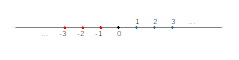
\includegraphics[width=0.8\textwidth]{./cap_numreal/dados/fig_reprgeoZ/main}
  \caption{Representação geométrica dos números inteiros.}
  \label{fig:reprgeoZ}
\end{figure}

\begin{ex}
  Consideramos os seguintes casos:
  \begin{enumerate}[a)]
  \item $-1$ é o oposto de $1$:
    \begin{equation}
      1 + (-1) = 0
    \end{equation}
  \item $2$ é o oposto de $-2$:
    \begin{equation}
      -2 + 2 = 0
    \end{equation}
  \end{enumerate}
\end{ex}

Os números inteiros contém os números naturais, i.e.
\begin{equation}
  \mathbb{N} \subset \mathbb{Z}.
\end{equation}
Ainda, as operações de \emph{adição} e \emph{multiplicação} podem ser imediatamente estendidas para os números inteiros, assim como suas \emph{propriedades} de \emph{elemento neutro}, \emph{comutatividade} e \emph{associatividade}.

\subsubsection{Operação de Subtração}

Com a definição de oposto, podemos definir a \emph{operação de subtração} de dois números inteiros da seguinte forma
\begin{gather}
  m - n = m + (-n) \\
  = -n + m,
\end{gather}
sendo a operação de adição definida usualmente.

\begin{ex}
  \begin{gather}
    2 - 3 = 2 + (-3) \\
    = -3 + 2 = -1
  \end{gather}

  \ifispython
  No \python, esta operação pode ser feita de forma usual
  \begin{lstlisting}
    In : 2 - 3
    Out: -1
  \end{lstlisting}
  \fi
\end{ex}

\ifispython
\begin{obs}
  No \sympy, o conjunto dos números inteiros é definido por \lstinline!S.Integers! e uma variável simbólica inteira pode ser definida com
  \begin{lstlisting}
    from sympy import *
    m = Symbols('m', integer=True)
  \end{lstlisting}
\end{obs}
\fi

\subsubsection{Valor absoluto}

Dada um número $p\in\mathbb{Z}$, definimos o seu \emph{valor absoluto}\footnote{Também, chamado de \emph{módulo} ou \emph{norma}.} pelo número inteiro
\begin{equation}\label{eq:racionais_abs}
  |p| = \left\{
    \begin{array}{ll}
      p &, p\geq 0,\\
        -p &, p<0.
    \end{array}
\right.
\end{equation}

\begin{ex}
  Estudemos os seguintes casos:
  \begin{enumerate}[a)]
  \item $|3| = 3$
  \item $|-2| = -(-2) = 2$
  \item $|0| = 0$
  \end{enumerate}
  \ifispython
  Com o {\sympy}, podemos computar estes casos como segue:
  \begin{lstlisting}
    >>> from sympy import *
    >>> Abs(-3)
    3
    >>> Abs(3)
    3
    >>> Abs(0)
    0
  \end{lstlisting}
  \fi
\end{ex}

Para qualquer $p\in\mathbb{Z}$, a operação de tomar o valor absoluto de um número tem as seguintes propriedades:
\begin{enumerate}[a)]
\item $|p|\geq 0$
\item $|p|=0\Leftrightarrow p=0$
\item $|p| = |-p|$
\item $|p|<q\Leftrightarrow -q<p<q$
\item $|p|>q\Leftrightarrow -p<-q\text{ ou }p>q$
\end{enumerate}

\subsection{Números racionais}

O conjunto dos números racionais é
\begin{equation}
  \mathbb{Q} = \left\{\frac{p}{q}:~p\in\mathbb{Z}\text{ e }q\in\mathbb{Z}^*\right\},
\end{equation}
sendo $\mathbb{Z}^*=\mathbb{Z}\setminus\{0\}$. O \emph{quociente} $p/q$ é definido como sendo o resultado da operação de \emph{divisão} de $p$ por $q$. Mais precisamente,
\begin{equation}
  \frac{p}{q} = x \Leftrightarrow p = x\cdot q.
\end{equation}

\begin{obs}
  Não está definida a \emph{divisão por zero}! Note que não existe $x$ tal que
  \begin{equation}
    \frac{p}{0} = x \Leftrightarrow p = 0\cdot x.
  \end{equation}
  Mesmo, $0/0$ não está bem definido. Neste caso, temos uma \emph{indeterminação matemática}, de fato não existe um único número $x$ tal que
  \begin{equation}
    \frac{0}{0} = x \Leftrightarrow 0 = 0\cdot x.
  \end{equation}
\end{obs}

A operação de \emph{adição} fica assim definida
\begin{equation}
  \frac{a}{b} + \frac{c}{d} = \frac{a\cdot d + b\cdot c}{b\cdot d}
\end{equation}

\begin{ex}
  \begin{gather}
    \frac{2}{5} + \frac{3}{4} = \frac{2\cdot 4 + 3\cdot 5}{5\cdot 4} \\
    = \frac{8 + 15}{20} \\
    = \frac{23}{20}
  \end{gather}

  \ifispython
  No \python, as operações são realizadas no conjunto dos números reais\footnote{Introduziremos os números reais na sequência.}\footnote{Mais precisamente, as operações são realizadas em ponto flutuante. Para mais informações, consulte \href{https://phkonzen.github.io/notas/MatematicaNumerica/cap_aritm.html}{aritmética de máquina}.}, por padrão. Por exemplo,
  \begin{lstlisting}
    In : 2/3
    Out: 1.5
  \end{lstlisting}
  Com o \sympy, podemos restringir a aritmética aos números racionais, com
  \begin{lstlisting}
    In : from sympy import S
    In : S(2)/3
    Out: 2/3
  \end{lstlisting}
  No caso do exemplo acima, temos
  \begin{lstlisting}
    In : S(2)/5 + S(3)/4
    Out: 23/20
  \end{lstlisting}
  \fi
\end{ex}

A operação de \emph{multiplicação} fica definida por
\begin{equation}
  \frac{a}{b}\cdot\frac{c}{d} = \frac{a\cdot c}{b\cdot d}.
\end{equation}

\begin{ex}
  \begin{gather}
    \frac{2}{5}\cdot\frac{3}{2} = \frac{\cancel{2}\cdot 3}{5\cdot \cancel{2}} \\
    = \frac{3}{5}
  \end{gather}

  \ifispython
  No \python, temos
  \begin{lstlisting}
    In : from sympy import S
    In : S(2)/5 * S(3)/2
    Out: 3/5
  \end{lstlisting}
  \fi
\end{ex}

\begin{obs}
  \begin{equation}
    \mathbb{N} \subset \mathbb{Z} \subset \mathbb{Q}
  \end{equation}
  Isso segue do fato de que se $m\in\mathbb{Z}$, então
  \begin{equation}
    m = \frac{m}{1}.
  \end{equation}
  
  Os números racionais também herdam as \emph{propriedades} de \emph{elemento neutro}, \emph{comutatividade} e \emph{associatividade} nas operações de adição e multiplicação.
\end{obs}

\subsubsection{Operação de Potenciação}

Outra operação fundamental é a operação de \emph{potenciação}. A potenciação de um número racional $p/q\neq 0$ por um número natural $n$ é definida por
\begin{equation}
  \left(\frac{p}{q}\right)^n = \underbrace{\frac{p}{q}\cdot\frac{p}{q}\cdot\cdots\cdot\frac{p}{q}}_{n\text{ vezes}},
\end{equation}
sendo $(p/q)^0 = 1$. Ainda, definimos o \emph{inverso de um número} racional $p/q$ por
\begin{equation}
  \left(\frac{p}{q}\right)^{-1} = \frac{q}{p}.
\end{equation}
Mais precisamente, o inverso de um número $x\neq 0$ é denotado por $x^{-1}$ e é tal que
\begin{equation}
  x\cdot x^{-1} = 1.
\end{equation}
Com a escolha acima, vemos que $(p/q)^{-1}=q/p$, pois
\begin{align}
  \frac{p}{q}\cdot\frac{q}{p} &= \frac{p\cdot q}{q\cdot p}\\
                              &= \frac{q\cdot p}{q\cdot p}\\
                              &= \frac{q}{q}\cdot\frac{p}{p}\\
                              &= 1\cdot 1 = 1.
\end{align}

\begin{ex}
  Verifiquemos os seguintes casos:
  \begin{enumerate}[a)]
  \item
    \begin{gather}
      \left(\frac{3}{2}\right)^3 = \frac{3}{2}\cdot\frac{3}{2}\cdot\frac{3}{2} \\
      = \frac{9}{4}\cdot\frac{3}{2} \\
      = \frac{27}{8}
    \end{gather}
  \item
    \begin{gather}
      2^3 = 2\cdot 2 \cdot 2 \\
      = 4\cdot 2\\
      = 8
    \end{gather}
  \item
    \begin{equation}
      \left(\frac{3}{2}\right)^{-1} = \frac{2}{3}
    \end{equation}
  \end{enumerate}

  \ifispython
  No \python, o operador de potenciação é \lstinline!**!. Os casos acima podem ser computados como segue
  \begin{lstlisting}
    In : from sympy import S
    In : (S(3)/2)**3
    Out: 27/8
    In : 2**3
    Out: 8
    In : (S(3)/2)**-1
    Out: 2/3
  \end{lstlisting}
  \fi
\end{ex}

\begin{obs}\label{obs:020}
  Enquanto que para $x\neq 0$ temos $x^0=1$, $0^0$ não está bem definida! Trata-se de uma \emph{indeterminação}, conceito normalmente introduzido em um curso de Cálculo. Por outro lado, há situações em que se adota-se a convenção de que $0^0=1$. Este é o caso da linguagem {\python} e várias outras.
  \ifispython
  Em {\python}, temos
  \begin{lstlisting}
    >>> 0**0
    1
  \end{lstlisting}
  \fi
\end{obs}

Sendo $a,b\in\mathbb{Q}$ e $n, m\in\mathbb{N}$, temos as seguintes \emph{propriedades} fundamentais da operação de potenciação\footnote{Estas propriedades são válidas desde que as operações estejam bem definidas. Por exemplo, a segunda propriedade elencada somente é válida no caso de $a\neq 0$.}:
\begin{itemize}
\item $a^{m+n} = a^m\cdot a^n$
\item $\displaystyle a^{-m} = \left(a^m\right)^{-1} = \left(a^{-1}\right)^m$
\item $\displaystyle a^{m\cdot n} = \left(a^m\right)^n = \left(a^n\right)^m$
\item $\displaystyle \left(\frac{a}{b}\right)^m = \frac{a^m}{b^m}$
\end{itemize}

\begin{obs}
  As seguintes potenciações não estão bem definidas:
  \begin{itemize}
  \item $\nexists ~0^{-1}$
    \begin{equation}
      0^{-1} = \cancelto{\nexists}{\frac{1}{0}}
    \end{equation}
    O símbolo $\exists$ lê-se existe e o $\nexists$ lê-se não existe.
    
  \item $\nexists ~0^0$

    \begin{gather}
      0^0 = 0^{1-1} \\
      = 0^1\cdot 0^{-1}\\
      = 0\cdot \cancelto{\nexists}{\frac{1}{0}}
    \end{gather}
  \end{itemize}
  Sobre este último caso, lembre-se da Observação \ref{obs:020}.
\end{obs}

\ifispython
\begin{obs}
  No \sympy, o conjunto dos números racionais é definido por \lstinline!S.Rationals! e uma variável simbólica racional pode ser definida com
  \begin{lstlisting}
    from sympy import *
    a = Symbols('a', rational=True)
  \end{lstlisting}
\end{obs}
\fi

\begin{obs}\label{obs:razao_irredutivel}
  A representatividade de números racionais não é única. Por exemplo,
  \begin{equation}
    \frac{2}{3} = \frac{4}{6} = \frac{14}{21} = \cdots
  \end{equation}
  Isto nos motiva a introduzir o conceito de \emph{razão irredutível}. Dizemos que $p/q$ é uma razão irredutível, quando $p$ e $q$ não têm divisor comum\footnote{Um número $m\in\mathbb{N}^*$ é divisor de $n\in\mathbb{Z}$, quando $m/n\in\mathbb{Z}$.}. Por exemplo, $2/3$ é uma razão irredutível, enquanto $4/6$ não é, pois $4$ e $6$ têm $2$ como divisor comum.
\end{obs}

\subsection*{Exercícios}

\begin{exer}
  Sejam $m,n,p,q\in\mathbb{N}$. Argumente se são verdadeiras ou falsas as seguintes afirmações:
  \begin{enumerate}[a)]
  \item $m = 0 + m$
  \item $m + (n + p) = (n + p) + m$
  \item $m + n + p = (n + m) + p$
  \item $(m+n) + (q + p) = (m + p) + (q + n)$
  \item $1\cdot m \neq m\cdot 1$
  \item $(m\cdot n)\cdot p = (n\cdot p)\cdot m$
  \end{enumerate}
\end{exer}
\begin{resp}
  a) V; b) V; c) V; d) V; e) F; f) V
\end{resp}

\begin{exer}
  Sejam $m,n,p,q\in\mathbb{Z}$. Argumente se são verdadeiras ou falsas as seguintes afirmações:
  \begin{enumerate}[a)]
  \item $n - p = p - n$
  \item $(m - n) + p = (m + p) - n$
  \item $-(-m) = m$
  \end{enumerate}
\end{exer}
\begin{resp}
  a) F; b) V; c) V
\end{resp}

\begin{exer}
  O \emph{mínimo múltiplo comum} dos números de dois números inteiros $c,d$ é denotado por $\mmc(c,d)$ e é o menor inteiro positivo que é múltiplo simultaneamente de $c$ e $d$. Sendo, ainda, $a,b\in\mathbb{Z}$ e $c,d\neq 0$, Mostre que
  \begin{equation}
    \frac{a}{c} + \frac{b}{d} = \frac{a\cdot\frac{\mmc(c,d)}{c}+b\cdot\frac{\mmc(c,d)}{d}}{\mmc(c,d)}.
  \end{equation}
  Qual a vantagem em usar o $\mmc$ para calcular a soma de frações?
  \ifispython
  No {\sympy}, pode-se utilizar o método \href{https://docs.sympy.org/latest/modules/core.html?highlight=lcm#ilcm}{\lstinline+sympy.ilcm+}. Verifique!
  \fi
\end{exer}
\begin{resp}
  Dica: $\displaystyle \frac{a}{c} + \frac{b}{d} = \frac{a\cdot d + b\cdot c}{c\cdot d}$
\end{resp}

\begin{exer}
  Sejam $p,q\in\mathbb{Q}$, $q\neq 0$, $m,n\in\mathbb{Z}$. Argumente sobre a veracidade das seguintes afirmações.
  \begin{enumerate}[a)]
  \item $q^{m-n} = \frac{q^m}{q^n}$
  \item $\displaystyle \left(\frac{p}{q}\right)^m = \frac{p^m}{q}$
  \item $q^{-m\cdot n} = \frac{q^n}{q^m}$
  \end{enumerate}
\end{exer}
\begin{resp}
  a) V; b) F; c) V
\end{resp}

\begin{exer}
  $1+1 = 1$? Encontre o erro nos seguintes cálculos:
  \begin{align}
    a &= b\\
    a^2 &= ab\\
    a^b - b^2 &= ab - b^2\\
    (a+b)(a-b) &= b(a-b)\\
    a+b &= b
  \end{align}
  Escolhendo, por exemplo, $a=1$ e $b=1$, esta última fornece $1+1 = 1$!
\end{exer}

\begin{exer}
  Seja $p,q\in\mathbb{Q}$. Mostre as seguintes propriedades:
  \begin{enumerate}[a)]
  \item $|p|\geq 0$
  \item $|p| = |-p|$
  \item $|p|<q\Leftrightarrow -q<p<q$
  \item $|p|>q\Leftrightarrow -p<-q\text{ ou }p>q$
  \end{enumerate}
\end{exer}
\begin{resp}
  Dica: Por definição, para $p\geq 0$ tem-se $|p|=p$ e, para $p<0$ tem-se $|p|=-1$. Consulte \eqref{eq:racionais_abs}.
\end{resp}

\section{Conjunto dos números reais}\label{cap_numreal_sec_numreal}

\subsection{Existência de números irracionais}

Para introduzirmos os números reais, vamos fazer a tentativa de estender a operação de potenciação para potências racionais. Mais especificamente, vamos tentar determinar $\sqrt{2}$, a qual é definida por
\begin{equation}
  \sqrt{2} = 2^{\frac{1}{2}}.
\end{equation}
Assumindo válidas as propriedades de potenciação vista para números racionais, teríamos
\begin{gather}
  \left(2^{\frac{1}{2}}\right)^2 = 2^{\frac{1}{2}\cdot 2} \\
  = 2^1 = 2.
\end{gather}
Será que $2^{\frac{1}{2}}$ é um número racional? Se fosse, então existiria uma \emph{razão irredutível}\footnote{Sobre razão irredutível, consulte a Observação \ref{obs:razao_irredutivel}.} $p/q$ tal que $2^{\frac{1}{2}} = p/q$, $p\in\mathbb{Z}$ e $q\in\mathbb{Z}^*$, com
\begin{gather}
  \left(\frac{p}{q}\right)^2 = 2 \\
  \Leftrightarrow\nonumber\\
  \frac{p^2}{q^2} = 2 \\
  \Leftrightarrow\nonumber\\
  p^2 = 2\cdot q^2.
\end{gather}
Logo, $p^2$ é um número par\footnote{Número múltiplo inteiro de $2$.} e, portanto, $p$ é um número par\footnote{O quadrado de um número ímpar é um número ímpar. Número ímpar é um número inteiro não divisível por $2$.}. Ou seja, existiria $m\in\mathbb{Z}$ tal que $p = 2m$. Mas, então
\begin{gather}
  (2\cdot m)^2 = 2\cdot q^2 \\
  \Leftrightarrow\nonumber\\
  4\cdot m^2 = 2\cdot q^2 \\
  \Leftrightarrow\nonumber\\
  2\cdot m^2 = q^2.
\end{gather}
Com isso, $q^2$ seria par e, portanto, $q$ deveria ser par. Isso é uma contradição, por $p/q$ é uma razão irredutível. Logo, concluímos que
\begin{equation}
  \sqrt{2}\not\in\mathbb{Q}.
\end{equation}
Assim sendo, dizemos que $\sqrt{2}$ é um \emph{número irracional}. Ou seja, não é racional! :D

\begin{obs}
  Uma aplicação em geometria. Observamos que $\sqrt{2}$ é o comprimento do lado do quadrado de área 1. Ou ainda, $\sqrt{2}$ é a hipotenusa do triângulo retângulo de catetos com comprimento igual a 1!
\end{obs}

\subsection{Fecho dos números racionais}

Mas então, como podemos calcular o número $\sqrt{2}$? Bem, podemos aproximá-lo usando o \href{https://en.wikipedia.org/wiki/Methods\_of\_computing\_square_roots#Babylonian\_method}{método babilônico}. Observamos que $\sqrt{2}$ é um número entre $1$ e $2$, exclusivamente. Vamos, então, escolher como aproximação inicial
\begin{equation}
  x_0 = \frac{3}{2} = 1.5
\end{equation}
Daí, calculamos uma nova aproximação como
\begin{gather}
  x_1 = \frac{1}{2}\left(x_0 + \frac{2}{x_0}\right) \\
  = \frac{1}{2}\left(\frac{3}{2} + \frac{2}{\frac{3}{2}}\right) \\
  = \frac{1}{2}\left(\frac{3}{2} + \frac{4}{3}\right) \\
  = \frac{1}{2}\left(\frac{9+8}{6}\right)\\
  = \frac{1}{2}\cdot\frac{17}{6} \\
  = \frac{17}{12} = 1,41\bar{6}
\end{gather}
Então, analogamente podemos calcular uma melhor aproximação com
\begin{gather}
  x_2 = \frac{1}{2}\left(x_1 + \frac{2}{x_1}\right) \\
  = \frac{1}{2}\left(\frac{17}{12} + \frac{2}{\frac{17}{12}}\right) \\
  = \frac{577}{408} = 1,41421\overline{5686274509803921}
\end{gather}
e assim sucessivamente. Estes números racionais estão de fato se aproximando do valor de $\sqrt{2}$. Notamos que
\begin{gather}
  x_0^2 = \left(\frac{3}{2}\right)^2 = 2,25\\
  x_1^2 = \left(\frac{17}{12}\right)^2 = 2,0069\bar{4} \\
  x_2^2 = \left(\frac{577}{408}\right)^2 = 2,000006\ldots
\end{gather}

O método babilônico, nos mostra que $\sqrt{2}$ pode ser calculado como o \emph{limite} de uma \emph{sequência} de números racionais. Ou seja, é sempre possível escolher um número racional que aproxime do valor de $\sqrt{2}$ tão bem quanto se queira. No caso, basta iterarmos o método babilônico um número suficiente de vezes.

Neste caso, ainda dizemos que $\sqrt{2}$ pertence ao \emph{fecho} dos números racionais, escrevemos
\begin{equation}
  \sqrt{2}\in\overline{\mathbb{Q}}.
\end{equation}
Mais precisamente, $x\in\overline{\mathbb{Q}}$ quando sempre é possível escolher um número racional $p/q\in\mathbb{Q}$ que aproxima o valor de $x$ tão bem quanto se queira.

O \emph{conjunto dos números reais} é denotado por $\mathbb{R}$ e é tal que
\begin{equation}
  \mathbb{R} = \overline{\mathbb{Q}}.
\end{equation}
Ou seja, é a união dos números racionais com os números irracionais que podem ser arbitrariamente aproximados por números racionais.

\begin{obs}
  \begin{equation}
    \mathbb{N}\subset\mathbb{Z}\subset\mathbb{Q}\subset\mathbb{R}
  \end{equation}
  Além disso, os números reais herdam as operações e suas propriedades dos números racionais.
\end{obs}

\begin{ex}
  Consideramos os seguintes casos:
  \begin{enumerate}[a)]
  \item todo número inteiro é um número real.
  \item todo número racional é um número real.
  \item $\sqrt{3}, \sqrt{5}, \sqrt{7}, \cdots$ são números reais.
  \item $\pi = 3,141592\ldots$ é um número real.

    O $\pi$ é a área da circunferência de raio 1.
  \end{enumerate}

  \ifispython
  No \python, estes exemplos podem ser verificados com
  \begin{lstlisting}
    >>> from sympy import *
    >>> S.Integers.is_subset(S.Reals)
    True
    >>> S.Rationals.is_subset(S.Reals)
    True
    >>> sqrt(3) in S.Reals
    True
    >>> sqrt(5) in S.Reals
    True
    >>> sqrt(7) in S.Reals
    True
    >>> pi in S.Reals
    True
  \end{lstlisting}
  \fi
\end{ex}

De posse dos números reais, vamos definir $m$-ésima raiz de um número $x\in\mathbb{R}$ por
\begin{equation}
  \sqrt[m]{x} = x^{\frac{1}{m}},
\end{equation}
sendo que quando $m=2$, escrevermos simplesmente $\sqrt{x}$.

\begin{obs}
  \begin{equation}
    \sqrt{-1}\not\in\mathbb{R}
  \end{equation}

  De fato, seja
  \begin{equation}
    x = \sqrt{-1},
  \end{equation}
  então
  \begin{equation}
    x^2 = -1.
  \end{equation}
  Entretanto, o quadrado que qualquer número real é um número não negativo! Ou seja, $x\not\in\mathbb{R}$.

  Mais geralmente, não é número real a raiz de índice par de qualquer número negativo.
\end{obs}

\subsection{Reta real}\label{ssec:numreal_retareal}

A reta real é uma representação geométrica do conjunto dos números reais (Figura \ref{fig:conjreal_retareal}).

\begin{figure}[H]
  \centering
  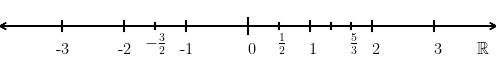
\includegraphics[width=0.9\textwidth]{./cap_numreal/dados/fig_retareal/fig_retareal}
  \caption{Reta real.}
  \label{fig:conjreal_retareal}
\end{figure}

Traçamos uma reta horizontal e escolhemos um ponto como sendo a origem. Neste ponto, marcamos a posição do número zero. Usando um espaçamento fixo, posicionamos os números naturais a direita do zero e de forma sucessiva. Os números inteiros negativos são posicionados à esquerda do zero, também em posições sucessivas. Os números racionais são posicionados tomando as frações do espaçamento escolhido. A Figura \ref{fig:conjreal_retareal} é um esboço da reta real.

Uma das propriedades notáveis dos números reais é a chamada \emph{tricotomia}, i.e. um número real $x$ é
\begin{itemize}
\item positivo (posicionado à direita da origem),
\item zero (posicionado na origem), ou
\item negativo (posicionado à esquerda da origem),
\end{itemize}
exclusivamente.

\subsection{Infinito}

O infinito é denotado por $\infty$ e representa a noção daquilo que não tem fim. Quando sem sinal, é interpretado na direção positiva (direita) da reta real. Quando escrito $-\infty$ (lê-se menos infinito) é interpretado na direção negativa (esquerda) da reta real. Nesta reta (Fig. \ref{fig:conjreal_retareal_infty}), $\infty$ é representado por sua seta à direta e $-\infty$ por sua seta à esquerda.

\begin{figure}[H]
  \centering
  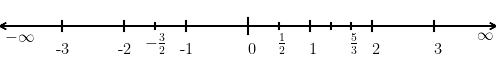
\includegraphics[width=0.9\textwidth]{./cap_numreal/dados/fig_retareal_infty/fig}
  \caption{Reta real.}
  \label{fig:conjreal_retareal_infty}
\end{figure}


\begin{obs}
  $\infty$ não é um número!
\end{obs}

Sendo $x$ é um número real, podemos inferir as seguintes propriedades para qualquer dado $x\in\mathbb{R}$:
\begin{itemize}
\item $\pm\infty \pm x = \pm\infty$ \\
\item $\pm\infty \mp x = \pm\infty$ \\
\item $-\infty = -1\cdot\infty$ \\
\item $x\cdot(\pm\infty) = \pm\infty$, $x>0$
\item $x\cdot(\pm\infty) = \mp\infty$, $x<0$
\item $\pm\infty \pm \infty = \pm\infty$ \\
\item $(\pm\infty)\cdot(\pm\infty) = \infty$ \\
\item $(\pm\infty)\cdot(\mp\infty) = -\infty$
\end{itemize}

\begin{ex}
  Estudamos os seguintes casos:
  \begin{enumerate}[a)]
  \item $\infty + \infty = \infty$
  \item $-1\cdot (-\infty) = \infty$
  \item $2\cdot (-\infty) = -\infty$
  \item $\infty\cdot\infty = \infty$
  \item $-\infty\cdot\infty = -\infty$
  \end{enumerate}

  \ifispython
  No \python, podemos verificar estas contas com os seguintes comandos:
  \begin{lstlisting}
    >>> from sympy import *
    >>> oo + oo
    oo
    >>> -1 * -oo
    oo
    >>> 2 * -oo
    -oo
    >>> oo * oo
    oo
    >>> -oo * oo
    -oo
  \end{lstlisting}
  \fi
\end{ex}

No entanto, são consideradas \emph{indeterminações matemáticas} as seguintes operações:
\begin{itemize}
\item $\infty - \infty$
\item $0\cdot\infty$
\item $\displaystyle\frac{\infty}{\infty}$
\item $\infty^0$
\item $1^\infty$
\item $0^0$
\item $\displaystyle\frac{0}{0}$
\end{itemize}

\ifispython
\begin{obs}
  Com o \sympy, as indeterminações são marcadas como \lstinline!nan!\footnote{Do inglês, {\it not a number}.} ou retornam erro. Por exemplo:
  \begin{lstlisting}
    >>> from sympy import *
    >>> oo - oo
    nan
    >>> 0/0
    Traceback (most recent call last):
    File "<stdin>", line 1, in <module>
    ZeroDivisionError: division by zero
  \end{lstlisting}
  Atenção! Exceções são os casos envolvendo potências de expoente $0$, por exemplo:
  \begin{lstlisting}
    >>> 0**0
    1
    >>> oo**0
    1
  \end{lstlisting}
\end{obs}
\fi

\subsection{Intervalos de números reais}

Intervalos de números reais são conjuntos especiais e muito utilizados. Por simplicidade, recebem uma notação própria. Para $a, b\in\mathbb{R}$, temos os seguintes tipos de intervalos:
\begin{itemize}
\item Intervalo fechado
  \begin{equation}
    [a, b] = \{x\in\mathbb{R}:~a\leq x\leq b\}
  \end{equation}

  \begin{figure}[H]
    \centering
    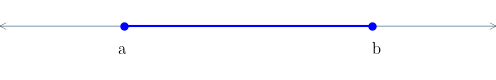
\includegraphics{./cap_numreal/dados/fig_int_fechado/main}
    \caption{Representação geométrica de um intervalo $[a,b]$.}
    \label{fig:intFechado}
  \end{figure}
  
\item Intervalo semi-aberto à esquerda (semi-fechado à direita)
  \begin{equation}
    (a, b] = \{x\in\mathbb{R}:~a< x\leq b\}
  \end{equation}  

  \begin{figure}[H]
    \centering
    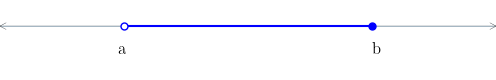
\includegraphics{./cap_numreal/dados/fig_int_semiaberto_esq/main}
    \caption{Representação geométrica de um intervalo $(a,b]$.}
    \label{fig:intSemiAbertoE}
  \end{figure}

  
\item Intervalo semi-aberto à direita (semi-fechado à esquerda)
  \begin{equation}
    [a, b) = \{x\in\mathbb{R}:~a\leq x< b\}
  \end{equation}  

  \begin{figure}[H]
    \centering
    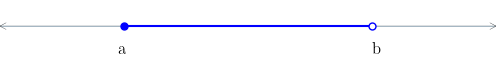
\includegraphics{./cap_numreal/dados/fig_int_semiaberto_dir/main}
    \caption{Representação geométrica de um intervalo $[a,b)$.}
    \label{fig:intSemiAbertoD}
  \end{figure}

\item Intervalo aberto
  \begin{equation}
    (a, b) = \{x\in\mathbb{R}:~a< x< b\}
  \end{equation}  

  \begin{figure}[H]
    \centering
    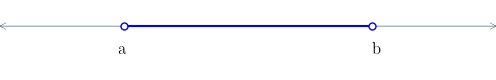
\includegraphics{./cap_numreal/dados/fig_int_aberto/main}
    \caption{Representação geométrica de um intervalo $(a,b)$.}
    \label{fig:intAberto}
  \end{figure}

\end{itemize}

\begin{ex}
  Vamos estudar os seguintes casos:
  \begin{enumerate}[a)]
  \item $-2\in [-3, 1]$
  \item $\displaystyle \sqrt{2}\in \left(1, \frac{3}{2}\right)$
  \item $2\not\in [-3, 2)$
  \item $\pi\in (3, 4]$
  \item $[a, a] = \{a\}$
  \item $[3, 2]=\emptyset$
  \item $(1, 1)=\emptyset$
  \end{enumerate}
  

  \ifispython
  Com o \sympy, podemos checar os casos acima usando o comando \href{https://docs.sympy.org/latest/modules/sets.html#sympy.sets.sets.Interval}{\lstinline{Interval}}. Vejamos alguns dos casos acima:
  \begin{lstlisting}
    >>> from sympy import *
    >>> -2 in Interval(-3, 1)
    True
    >>> sqrt(2) in Interval(1,3/2,
    ... left_open=True, right_open=True)
    True
    >>> 2 in Interval(-3,2,right_open=True)
    False
    >>> Interval(3,2)
    EmptySet
  \end{lstlisting}
  \fi
\end{ex}

Ainda, temos os seguintes casos especiais
\begin{itemize}
\item Intervalos semi-limitados à esquerda
  \begin{gather}
    [a, \infty) = \{x\in\mathbb{R}:~a\leq x\}
    (a, \infty) = \{x\in\mathbb{R}:~a< x\}
  \end{gather}

  \begin{figure}[H]
    \centering
    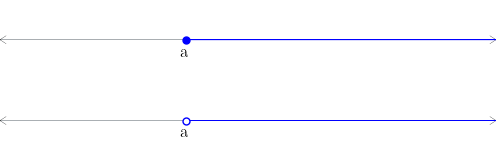
\includegraphics{./cap_numreal/dados/fig_int_semilimitados_esq/main}
    \caption{Representação geométrica dos intervalos $[a,\infty)$ (acima) e $(a,\infty)$ (abaixo).}
    \label{fig:intSemiLimitadosE}
  \end{figure}
  
\item Intervalos semi-limitados à direita
  \begin{gather}
    (-\infty, b] = \{x\in\mathbb{R}:~x\leq b\}
    (-\infty, b) = \{x\in\mathbb{R}:~x< b\}
  \end{gather}

  \begin{figure}[H]
    \centering
    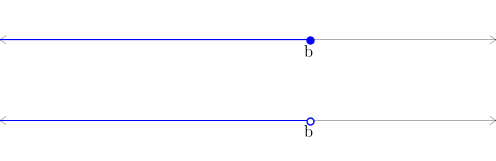
\includegraphics{./cap_numreal/dados/fig_int_semilimitados_dir/main}
    \caption{Representação geométrica dos intervalos $(-\infty, b]$ (acima) e $(-\infty, b)$ (abaixo).}
    \label{fig:intSemiLimitadosD}
  \end{figure}

\item Intervalo ilimitado
  \begin{equation}
    (-\infty, \infty) = \mathbb{R}
  \end{equation}

  \begin{figure}[H]
    \centering
    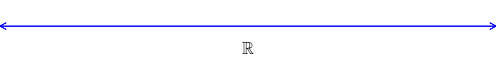
\includegraphics{./cap_numreal/dados/fig_int_ilimitado/main}
    \caption{Representação geométrica dos intervalos $(-\infty, \infty)$.}
    \label{fig:intSemiLimitadosD}
  \end{figure}  
\end{itemize}

\begin{ex}
  Estudamos os seguintes casos:
  \begin{enumerate}[a)]
  \item $2\in [2, \infty)$
  \item $10^6\in (2, \infty)$
  \item $1 \not\in (-\infty, 1)$
  \item $-10^{308} \in (-\infty, 1]$
  \item $\pi \in (-\infty, \infty)$
  \end{enumerate}
  \ifispython
  Com o \python, podemos fazer estas verificações com os seguintes comandos:
  \begin{lstlisting}
    >>> from sympy import *
    >>> oo in Interval(2,oo)
    False
    >>> from sympy import *
    >>> 2 in Interval(2,oo)
    True
    >>> 10**6 in Interval(2,oo,
    ... left_open=True)
    True
    >>> 1 in Interval(-oo, 1,
    ... right_open=True)
    False
    >>> -10**308 in Interval(-oo, 1)
    True
    >>> pi in Interval(-oo, oo)
    True
  \end{lstlisting}
  \fi
\end{ex}

\subsection*{Exercícios}

\begin{exer}
  Verifique a veracidade de cada uma das seguintes afirmações. Justifique sua resposta.
  \begin{enumerate}[a)]
  \item Se $p,q$ são números pares, então $p+q$ é um número par.
  \item Se $p,q$ são números ímpares, então $p+1$ é um número ímpar.
  \item Se $p$ é número par e $q$ é número ímpar, então $p+q$ é número ímpar.
  \item Se $p$ é número par e $q$ é número ímpar, então $p\cdot q$ é número ímpar.
  \item Se $p,q$ são números ímpares, então $p\cdot q$ é número ímpar.
  \end{enumerate}
\end{exer}
\begin{resp}
  a) V; b) F; c) V; d) F; e) V
\end{resp}

\begin{exer}
  Mostre que $\sqrt{3}\not\in\mathbb{Q}$.
\end{exer}

\begin{exer}
  Um número primo $p$ tem somente quatro divisores $\pm 1$, $\pm p$ e é tal que $p\neq 0$ e $p\neq \pm 1$. Faça a \emph{decomposição em fatores primos} dos seguintes números\footnote{Dica: consulte o método \lstinline+sympy.factorint+.}.
  \begin{enumerate}[a)]
  \item $14$
  \item $24$
  \item $36$
  \item $2205$
  \end{enumerate}
\end{exer}
\begin{resp}
  a) $14 = 2\cdot 7$; b) $24 = 2^3\cdot 3$; c) $36 = 2^2\cdot 3^2$; d) $2205 = 3^2\cdot 5\cdot 7^2$
\end{resp}

\begin{exer}
  Encontre o resultado e faça a representação gráfica em cada um dos seguintes itens.
  \begin{enumerate}
  \item $(-1,2]\cup [-1,0]$
  \item $[2,4)\cap [4,5)$
  \item $(-2,2)\cap [-1,1)$
  \item $(-\infty, 1)\cup [0,\infty)$
  \item $(-1,1)\cup \{1\}$
  \end{enumerate}
\end{exer}
\begin{resp}
  a) $[-1,2]$, b) $\emptyset$; c) $[-1,1)$; d) $\mathbb{R}$; e) $(-1,1]$
\end{resp}

\begin{exer}
  Verifique a veracidade de cada uma das seguintes afirmações. Justifique sua resposta.
  \begin{enumerate}[a)]
  \item $\sqrt{2} + \sqrt{3} = \sqrt{5}$
  \item $\sqrt{4} + 2 = 4$
  \item $\sqrt{2}\cdot\sqrt{14} = 2\sqrt{7}$
  \item $\left(\sqrt{2})^3\right)=\sqrt{2^3}$
  \item $\sqrt[3]{2^2}=\sqrt[2]{2^3}$
  \end{enumerate}
\end{exer}
\begin{resp}
  a) F; b) V; c) V; d) V; e) F
\end{resp}

\begin{exer}
  Mostre que\footnote{$|x|=x$, $x\geq0$ e $|x|=-x$, caso contrário.} $\sqrt{x^2}=|x|$.
\end{exer}